\documentclass[uplatex,dvipdfmx,a4paper,11pt]{jsarticle}

\usepackage{docmute}


% 数式
\usepackage{amsmath,amsthm,amssymb}
\usepackage{bm}
% 画像
\usepackage{graphicx}

\usepackage{multirow}
\usepackage{wrapfig}
\usepackage{ascmac}
\usepackage{xcolor}


\usepackage{makeidx}
\makeindex

\graphicspath{{../../_Figures//}{../../_Figures/Rheology/}}

\usepackage{qrcode}
\setlength\lineskiplimit{0pt}
\setlength\normallineskiplimit{0pt}

\usepackage{qexam}

\usepackage{titlesec}
\titleformat*{\section}{\Large\bfseries}
\titleformat*{\subsection}{\large\bfseries}
\titleformat*{\subsubsection}{\normalsize\bfseries}
\titleformat*{\paragraph}{\normalsize\bfseries}

% ページ設定
% \pagestyle{empty}
% 高さの設定
\setlength{\textheight}{\paperheight}   % ひとまず紙面を本文領域に
\setlength{\topmargin}{-5.4truemm}      % 上の余白を20mm(=1inch-5.4mm)に
\addtolength{\topmargin}{-\headheight}  % 
\addtolength{\topmargin}{-\headsep}     % ヘッダの分だけ本文領域を移動させる
\addtolength{\textheight}{-40truemm}    % 下の余白も20mmに%% 幅の設定
\setlength{\textwidth}{\paperwidth}     % ひとまず紙面を本文領域に
\setlength{\oddsidemargin}{-5.4truemm}  % 左の余白を20mm(=1inch-5.4mm)に
\setlength{\evensidemargin}{-5.4truemm} % 
\addtolength{\textwidth}{-40truemm}     % 右の余白も20mmに
% 図と本文との間
%\abovecaptionskip=-5pt
%\belowcaptionskip=-5pt
%
% 全体の行間調整
% \renewcommand{\baselinestretch}{1.0} 
% 図と表
%\renewcommand{\figurename}{Fig.}
%\renewcommand{\tablename}{Tab.}
%

% \makeatletter 
% \def\section{\@startsection {section}{1}{\z@}{1.5 ex plus 2ex minus -.2ex}{0.5 ex plus .2ex}{\large\bf}}
% \def\subsection{\@startsection{subsection}{2}{\z@}{0.2\Cvs \@plus.5\Cdp \@minus.2\Cdp}{0.1\Cvs \@plus.3\Cdp}{\reset@font\normalsize\bfseries}}
% \makeatother 

\usepackage[dvipdfmx,%
 bookmarks=true,%
 bookmarksnumbered=true,%
 colorlinks=false,%
 setpagesize=false,%
 pdftitle={数式に頼らない直感的理解による材料設計のためのレオロジー⼊⾨},%
 pdfauthor={佐々木裕},%
 pdfsubject={},%
 pdfkeywords={レオロジー; 材料設計; }]{hyperref}
\usepackage{pxjahyper}

\usepackage{plext}

\usepackage{niceframe} 
\usepackage{framed}
\newenvironment{longartdeco}{%
  \def\FrameCommand{\fboxsep=\FrameSep \artdecoframe}%
  \MakeFramed {\FrameRestore}}%
 {\endMakeFramed}
 
\usepackage{siunitx}

\newcommand{\rmd}{\mathrm{d}}

\usepackage[inline]{showlabels}

\begin{document}

\question{演習問題 1}
内容を振り返るために、以下に示した文章例の中から適切な記述のものを複数選んでください。
	\begin{qlist}
		\qitem 力と釣り合いについての、正しい言葉はどれでしょうか?
		\begin{qlist2}
			\qitem 静力学とは、相互作用する物体系の運動について議論します。
			\qitem 物質に力を加えたとき、物質の内部には外力の何倍もの大きな力が生じます。
			\qitem 力とは、物体の状態を変化させる原因となる作用で、その作用の大きさを表す物理量と考えられます。
			\qitem 力の釣り合いを議論するものが静力学です。
			\qitem 作用した力と釣り合う力が生じることを、「作用・反作用の原理」といいます。
		\end{qlist2}
    \vspace{3mm}
    \begin{itembox}[l]{解答}
        正しい選択肢:(c), (d), (e)\\
        (解説)
		\begin{itemize}
			\item 静力学とは、時間によって系の位置が変化しない静的な状態で物体に働く力に関して議論するものでした。
			\item したがって、静力学で力の釣り合いを議論すれば、外力と内力が釣り合っていることや作用・反作用の原理がイメージできます。
		\end{itemize}
    \end{itembox}
	\qitem 「力学的な刺激と応答」についての、正しい言葉はどれでしょうか?
		\begin{qlist2}
			\qitem 物質に刺激を与えるということは変形させるということに対応し、変形の結果として応力という応答が生じます。
			\qitem ひずみとは、変形の状態を表す尺度であり、初期状態からどれだけ変位したかを表す無次元量です。
			\qitem ひずみとは、変形度合いを表す長さの次元を持った物理量です。
			\qitem 物質に加えた外力と応力とは、力の大きさを表す全く同一の物理量です。
			\qitem 応力の表す意味は単位面積あたりに働く内部の力ということになります。
		\end{qlist2}
    \vspace{3mm}
    \begin{itembox}[l]{解答}
        正しい選択肢:(a), (b), (e)\\
        (解説)
		\begin{itemize}
			\item 応力とは、外力と釣り合って物質の内部に生じている力の大きさを表す物理量です。
			\item したがって、外力とは異なり単位面積あたりに働く内部の力になります。
		\end{itemize}
    \end{itembox}
	\qitem 弾性体のモデルについての、正しい言葉はどれでしょうか?
		\begin{qlist2}
			\qitem 弾性体であっても、いったん外力により変形すると、もう元には戻りません。
			\qitem 弾性体はあたかもバネのように取り扱うことができます。
			\qitem 弾性体を表すモデルはニュートンの法則であり、ダッシュポットでイメージできます。
			\qitem 弾性体のフックモデルでは全体のひずみに比例するのは応力です。
			\qitem フックモデルでの比例定数が弾性率であり、応力と同じ次元 [Pa] です。
		\end{qlist2}
    \vspace{3mm}
    \begin{itembox}[l]{解答}
        正しい選択肢:(b), (d), (e)\\
        (解説)
		\begin{itemize}
			\item 弾性体はあたかもバネのように取り扱え、変形後も外力を除けばもとに戻ります。
			\item 弾性体を表すモデルはフックモデルであり、ひずみと応力が比例することを表します。
		\end{itemize}
    \end{itembox}
	\qitem 「液体の変形と応答」についての、正しい言葉はどれでしょうか?
	\begin{qlist2}
		\qitem 液体は、「外力によって変形されたら元には戻れない」流れるという性質を持った物質です。
		\qitem 液体に変形を与えると流れ、変形を止めれば応力も消えます。
		\qitem いったん変形を加えると、液体内部での応力はずっと維持されます。
		\qitem 液体は、変形させる速度が変わると生じる応力も変わります。
		\qitem 水中ではゆっくり歩いても水の抵抗は変化しません。
	\end{qlist2}
  \vspace{3mm}
  \begin{itembox}[l]{解答}
    正しい選択肢:(a), (b), (d)\\
    (解説)
	\begin{itemize}
		\item 液体は流れるという声質を持っていて、変形を止めれば応力も消えます。
		\item また、水中でゆっくり歩くと水の抵抗は小さくなり、これがニュートンの法則の「応力は変形速度に比例する」ことに対応します。
	\end{itemize}

\end{itembox}
	\qitem 液体のモデルについての、正しい言葉はどれでしょうか?
	\begin{qlist2}
		\qitem 液体の流れるという性質は、ニュートンの法則で整理できます。
		\qitem 液体はせん断速度に反比例してせん断応力が低下します。
		\qitem せん断応力は、せん断速度に比例します。
		\qitem 物質の流れやすさを表す指標である粘度は、測定条件に応じて常に変化します。
		\qitem 液体の力学モデルは、ダッシュポットで表されます。
	\end{qlist2}
    \vspace{3mm}
    \begin{itembox}[l]{解答}
    正しい選択肢:(a), (c), (e)\\
    (解説)
	\begin{itemize}
		\item 液体の性質は、基本的にはニュートンの法則に従います。
		\item 液体はせん断速度に比例して応力が大きく、すなわち、流れにくくなります。
		\item また、物質の流れやすさは粘度という比例定数で表されてせん断速度には依りません。
	\end{itemize}
    \end{itembox}
\end{qlist}

\question{演習問題 2}
内容を振り返るために、テキストで用いた言葉を使って簡単な穴埋めを行ってください。

\begin{qparts}
\qpart 「弾性体の力学的な刺激と応答」について、以下の\qbox{(a)}から\qbox{(i)}までのカッコを埋めてください。
		\begin{qlist}
			\qitem 変形は、物質を一つの軸に沿って引き伸ばす「\qbox{}」とトランプのカードを横にずらしたような「\qbox{}」の二つに単純化できます。
			\qitem 伸張変形では、\qbox{}を\qbox{}で除したものがひずみとなります。
			\qitem 応力とは、物質の内部に生じている\qbox{}を表す物理量であり、その表す意味は単位面積あたりの\qbox{}ということになります。
			\qitem 応力と力の関係は以下のように書けます。
			\begin{align*}
				\qbox{} = \dfrac{\qbox{}}{\qbox{}}
			\end{align*}
			% \qitem 一様な太さの棒を引っ張ったとき、棒の長手方向にはどの位置で切断したとしても、\qbox{}が働いていることに注意してください。

      \begin{itembox}[l]{選択肢}
        \begin{center}
          \begin{tabular}{lllll}
            1. 変形量	&2. せん断変形	&3. 力の大きさ	&4. 面積	&5. 応力\\
            6. 初期長さ	&7. 力		&8. 伸張変形				&9. 内部の力
          \end{tabular}
        \end{center}
      \end{itembox}

    \end{qlist}

\qpart 弾性体と液体の力学応答について、以下の\qbox{(j)}から\qbox{(p)}までのカッコを埋めてください。
		\begin{qlist}
			\qitem 弾性体を表すモデルはフックの法則であり、以下のように書けます。
				\begin{center}
					\begin{minipage}{0.45\textwidth}
						\begin{itemize}
							\item \qbox{} $\varepsilon$ と比例して、
							\item \qbox{} $\sigma$ が生じ、
							\item 比例定数が\qbox{} $E$
						\end{itemize}
						\begin{align*}
							\sigma = E \varepsilon
						\end{align*}
					\end{minipage}
					\begin{minipage}{0.35\textwidth}
						\begin{center}
						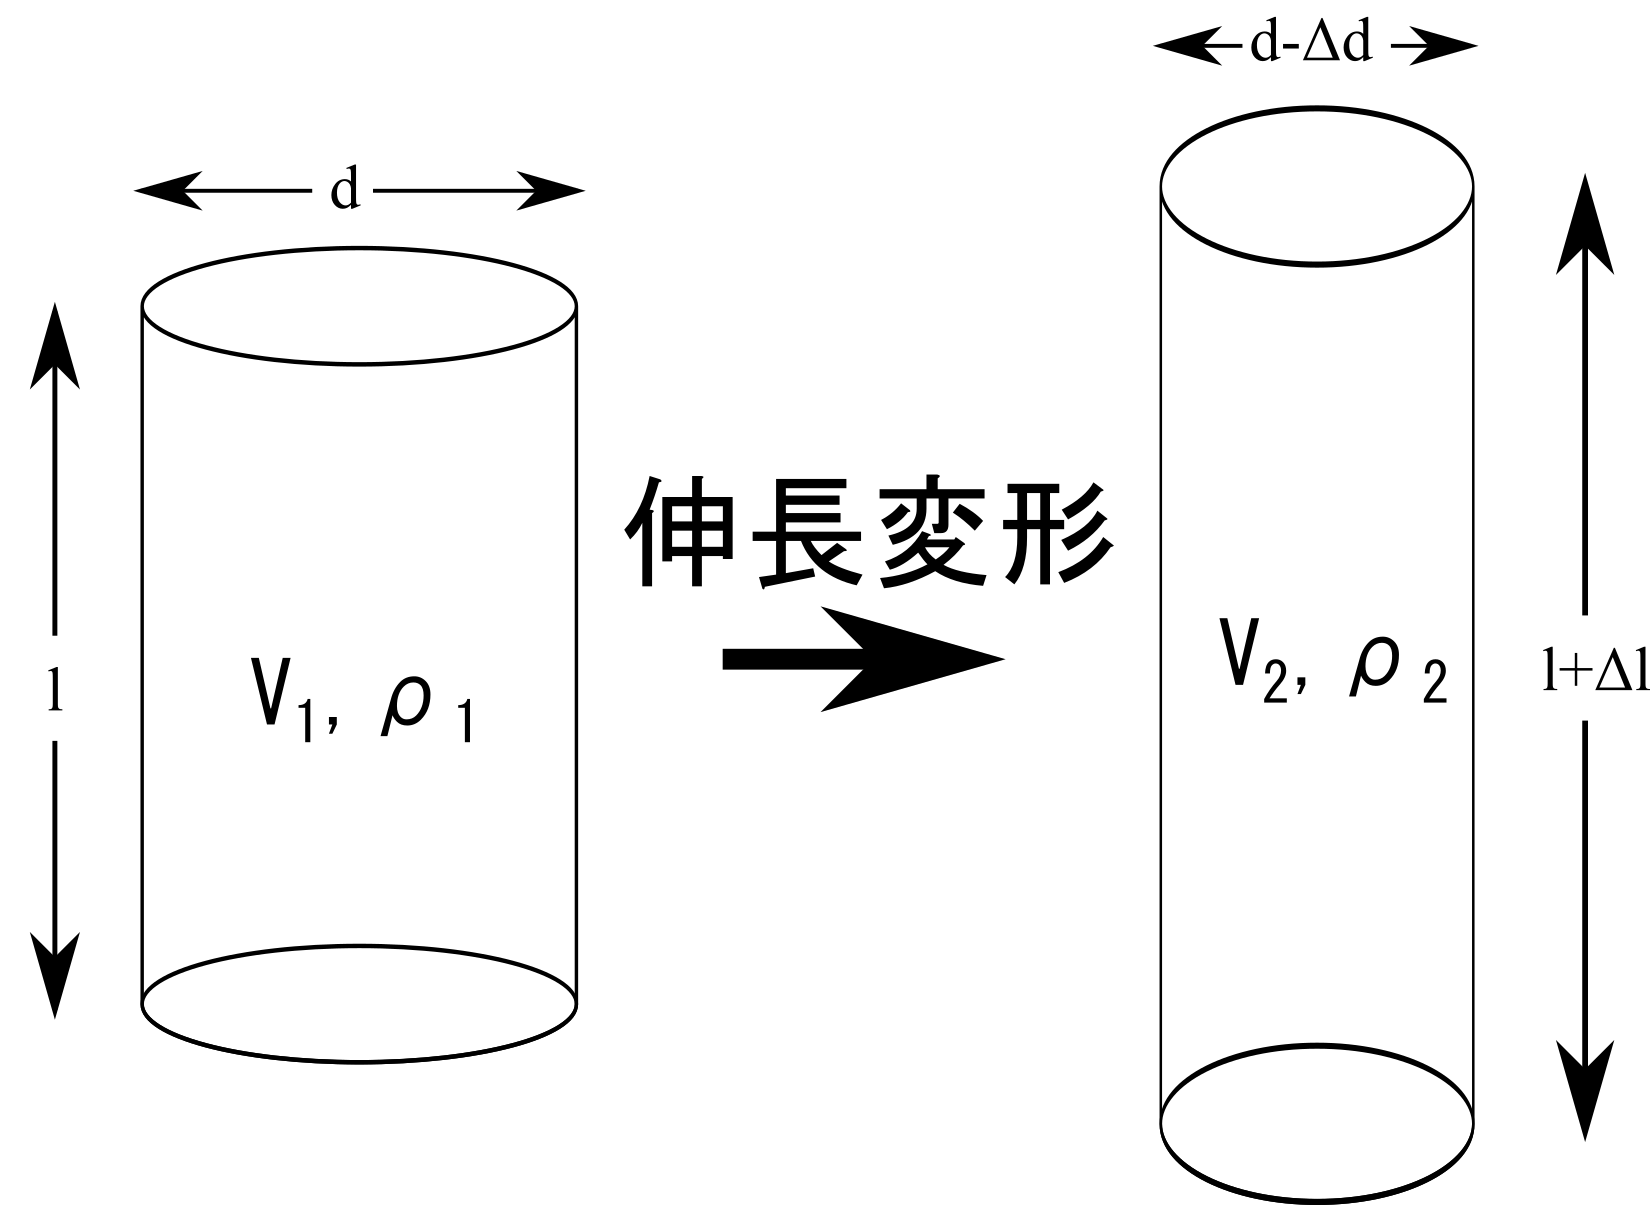
\includegraphics[width=.8\textwidth]{hook_law.png}
						\end{center}
					\end{minipage}
				\end{center}
			\qitem 液体の評価は主としてそのひずみ速度を維持しやすい「\qbox{}」により行われる場合が多くなります。
			\qitem ニュートンの法則の比例関係を式で表せば以下のようになります。
			\begin{align*}
				\text{\qbox{}} &= \text{\qbox{}} \times \text{\qbox{}} \notag \\
				\tau &= \eta \dot{\gamma}
      \end{align*}
      
      \begin{itembox}[l]{選択肢}
        \begin{center}
          \begin{tabular}{llll}
            1. 伸張弾性率	&2. ひずみ速度	&3. 伸張ひずみ	&4. せん断応力\\
            5. 伸張応力 	&6. せん断変形	&7. 粘度		
          \end{tabular}
        \end{center}
      \end{itembox}
  \end{qlist}

  \begin{itembox}[l]{解答}
    \begin{center} 
        \begin{tabular}{|p{.08\textwidth}|p{.08\textwidth}|p{.08\textwidth}|p{.08\textwidth}|p{.08\textwidth}|p{.08\textwidth}|p{.08\textwidth}|p{.08\textwidth}|} \hline
          (a) & (b) & (c) & (d) & (e) & (f) & (g) & (h)\\ \hline
            8 & 2 & 1 & 6 & 3 & 9 & 5 & 7 \\ \hline		
            (i) & (j) & (k) & (l) & (m) & (n) & (o) & (p)\\ \hline
            4 & 3 & 5 & 1 & 6 & 4 & 7 & 2 \\ \hline		
        \end{tabular}
      \end{center}
\end{itembox}

\end{qparts}

\question{演習問題 3}
数行程度の簡単な記述で構いませんので、以下の自由記述問題を考えてみてください。
\begin{qlist}
\qitem この章では、レオロジーのはじめの一歩として、その力学モデルについて簡単な説明を行ってきました。
弾性体と液体の力学モデルの特徴についてそれぞれ簡単にまとめて、その大きな違いについて書いてみてください。
\end{qlist}

\begin{itembox}[l]{解答例}
    固体は、弾性体としてモデル化することが出来て、これは、変形したとしても完全にもとに戻ることができるものとしてモデル化されています。
    したがって、バネのように取り扱うことが出来て、ひずみに比例した応力が発生します。

    一方、液体は、「外力によって変形されたら元には戻れない」流れるという性質を持った物質です。
    この力学モデルは、ニュートンの法則で記述されて、変形時に生じる応力はひずみ速度に比例することになります。
    \end{itembox}

\clearpage

\end{document}